\documentclass[]{paper}

\usepackage{graphicx}
\usepackage{float}

\begin{document}
\title{Minecraft Pi: Learning Python}
\author{Chris Gwilliams}
\date{\today}
\maketitle

\section*{What Are We Doing?}
Today, we are learning about the Python programming language through the glorious medium of VIDEO GAMING! As well as that, we will be using a Raspberry Pi.
\subsection*{How?}
Minecraft is an open-world procedural game made using the Java programming language and we can play it using a mouse and a keyboard. 
\subsection*{So?}
Minecraft can also be accessed through an Application Programming Interface (API) and we will be using one of the more awesome languages (Python) to mess about with the game while we play it.
\subsection*{Break it Down for Me}
\begin{enumerate}
	\item Play Minecraft
	\item Read some code
	\item Write some code
	\item Mess with Minecraft
	\item Use the Raspberry Pi
\end{enumerate}

\section{Setting Up}
Get into groups and huddle round your Raspberry Pi. What is that you say? It is still in bits? Well, this is task 1. Connect the right pieces to the Pi and turn that sucker on. You have 5 minutes, GO!
\subsection*{Hints}
 	The Raspberry Pi is powered like a mobile phone, stores its Operating System on an SD card and you cannot access it without a keyboard and some way of outputting its display. See Figure \ref{fig:rpi}.

\begin{figure}[H]
    \centering
    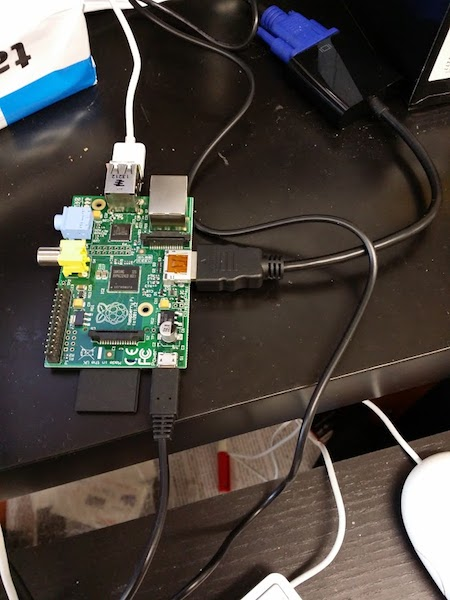
\includegraphics[width=0.8\textwidth]{figures/rpi.jpg}
    \caption{The Finished Piece}
    \label{fig:rpi}
\end{figure}

\section{Start Your Games}
Take some time to get acquainted with the software, looks a bit like Windows, right? This is an open-source OS, called Linux. On the desktop is a folder called \textbf{mcpi}, double click on that and this is what we will be using today. See Figure \ref{fig:mcpi}.

\begin{figure}[H]
    \centering
    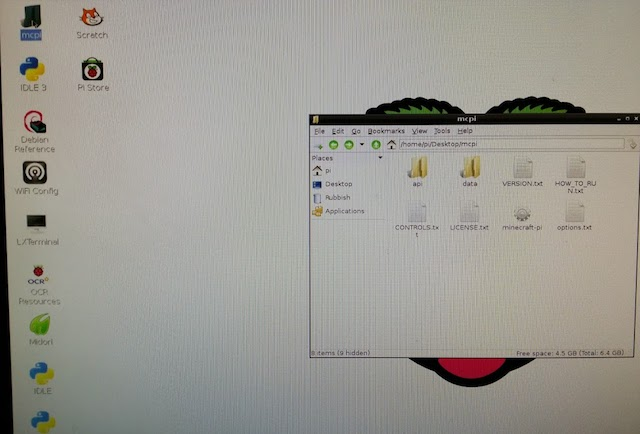
\includegraphics[width=0.8\textwidth]{figures/folder.jpg}
    \caption{MCPI Folder}
    \label{fig:mcpi}
\end{figure}

Inside that folder is a file called \textbf{minecraft-pi}, double click that and then select 'Execute' (Figure \ref{fig:mc}. WHAMMY, Minecraft is running! Go ahead and 'Start Game', then create a new world. This will take some time at first. Now use the controls below to go crazy!

\begin{figure}[H]
    \centering
    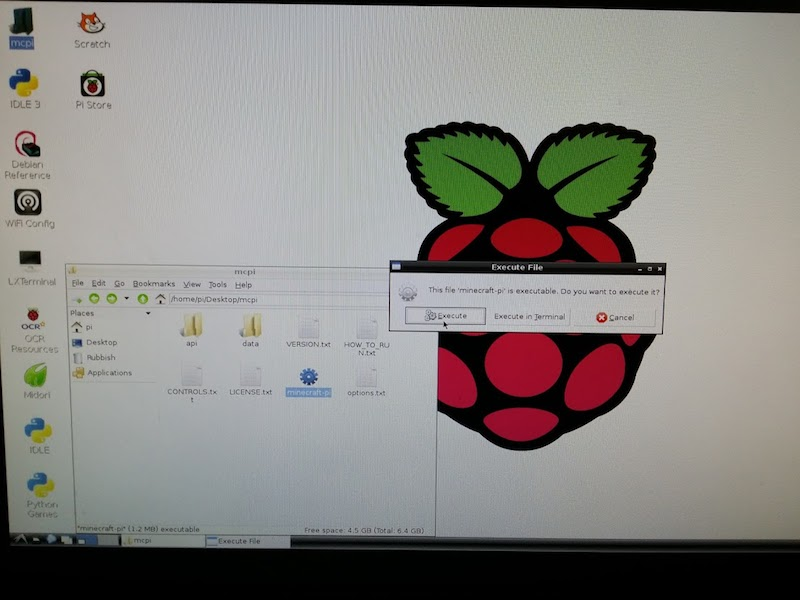
\includegraphics[width=0.8\textwidth]{figures/run-mc.jpg}
    \caption{Execute Minecraft}
    \label{fig:mc}
\end{figure}


\subsection*{Controls}
\begin{description}
	\item[WASD]: Forward, Left, Right and Back
	\item[Space]: Jump
	\item[Space (Double Tap)]: Fly
	\item[Space (Hold while flying)]: Go higher
	\item[Shift (While flying)]: Go lower
	\item[Mouse Movement]: Look around
	\item[Mouse Left Click]: Destroy block/Select item
	\item[Mouse Right Click]: Place currently selected item
	\item[E]: Open Inventory
\end{description}

\section{Using IDLE}
Had some fun with that? Now let's try messing about with the game! In the \textbf{mcpi} folder, click on \textbf{api} and then \textbf{python}. There should be a load of files in there. Right click on \textbf{demo\_chat.py} and open it with IDLE (Figure \ref{fig:idle}).

\begin{figure}[H]
    \centering
    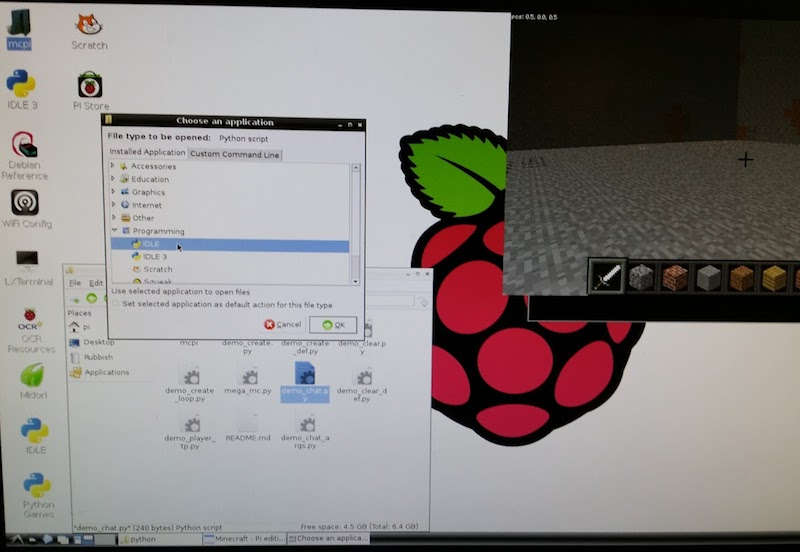
\includegraphics[width=0.8\textwidth]{figures/idle.jpg}
    \caption{Open With...IDLE}
    \label{fig:idle}
\end{figure}


We see a file full of code pop up and we will explain what it does. When you want to run it, click \textbf{Run} and then \textbf{Run Module} (Figure \ref{fig:run}).

\begin{figure}[H]
    \centering
    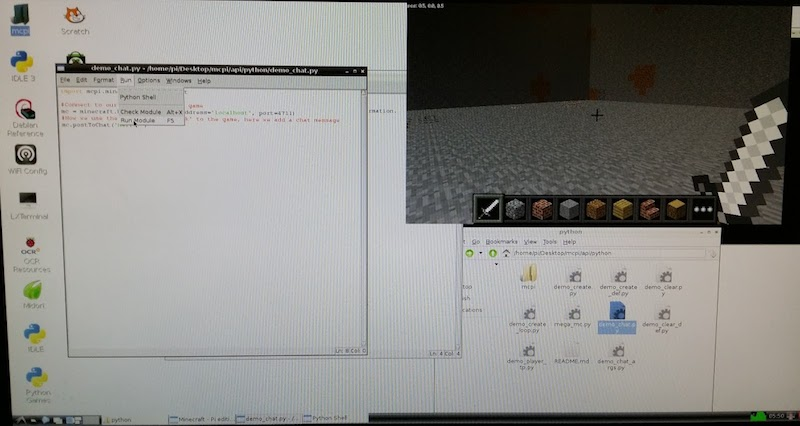
\includegraphics[width=0.8\textwidth]{figures/run.jpg}
    \caption{Run Module}
    \label{fig:run}
\end{figure}


You can do the same with some of the other files, open the following files and write down what they do:
\begin{itemize}
	\item \textbf{demo\_clear.py}
	\item \textbf{demo\_clear\_def.py}
	\item \textbf{demo\_create.py}
	\item \textbf{demo\_create\_def.py}
	\item \textbf{demo\_create.py}
	\item \textbf{demo\_player\_tp.py}
	\item \textbf{mega\_mc.py}
\end{itemize}

\subsection{Trivia!}
When you run one file in IDLE, nothing happens. Which file is it? Why do you think that is?

\section{GO CRAZY}
You have played the game. You have run the files. Now have a read of the comments and edit them.

\subsection*{Hints}
To play it safe, edit numbers and see what changes. Once you feel comfortable, mess about with variables and most important: DO NOT WORRY ABOUT BREAKING THE CODE OR THE GAME! That is the aim of today.

\section{Extra Credit}
Remember that file that did nothing when we ran it? Well, let's find out why. Follow these steps to the letter:
\begin{enumerate}
	\item Double click \textbf{LXTerminal} on the desktop
	\item Type '\textbf{cd Destkop/mcpi/api/python}' and press Enter
	\item Type '\textbf{python demo\_chat\_args.py hello}' and press Enter
\end{enumerate}
What happened? What happens if you change the word hello to something else? What do you think args stands for?

\section*{FINISHED!}
TA-DA! You have successfully:
\begin{enumerate}
	\item Set up a Raspberry Pi
	\item Used the Linux OS
	\item Played Minecraft!
	\item Used the Python programming language
\end{enumerate}

\end{document}